% Adapted from orx figures/assets/orx-tikz-preamble.tex.
% Serif fonts follow the user's manuscript-wide font requirement.
\documentclass[10pt]{article}
\usepackage[T1]{fontenc}
\usepackage[paperwidth=4.8in,paperheight=2.6in,margin=0pt]{geometry}
\usepackage{amsmath,tikz}
\usetikzlibrary{arrows.meta,positioning,fit,backgrounds,calc,shapes.geometric}
\definecolor{orxblue}{HTML}{0072B2}
\pagestyle{empty}\setlength\parindent{0pt}
\tikzset{
 orx/.style={font=\fontsize{8}{9.5}\selectfont,
  >={Stealth[round,length=4pt,width=3pt]},line width=.5pt},
 block/.style={draw=black!45,fill=white,rounded corners=1pt,inner sep=3pt,align=center},
 data/.style={block,fill=black!5,minimum width=10mm,minimum height=7mm},
 ours/.style={block,draw=orxblue,fill=orxblue!6,line width=.7pt},
 flow/.style={->,draw=black!65},
 stage/.style={draw=black!40,dashed,rounded corners=3pt,inner sep=3mm},
 latent/.style={circle,draw=black!65,fill=white,minimum size=2.7mm,inner sep=0pt},
 agent/.style={circle,draw=black!50,fill=white,minimum size=5.5mm,inner sep=0pt},
 label/.style={font=\fontsize{7.5}{9}\selectfont,align=center,inner sep=1pt},
 zoom/.style={draw=black!30,dashed,line width=.4pt}}
\begin{document}
\begin{minipage}[c][2.6in][c]{4.8in}\centering
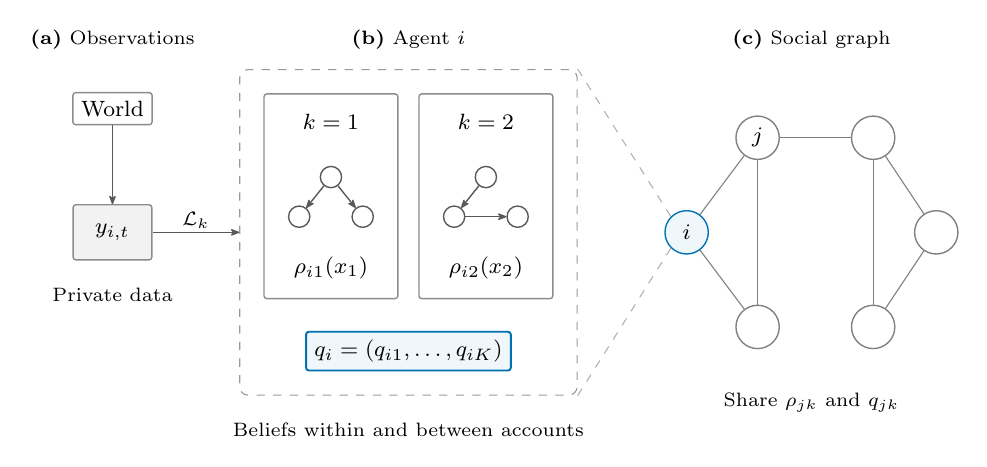
\begin{tikzpicture}[orx]
 \node[block,minimum width=17mm,minimum height=26mm] (c1)
  {\begin{tabular}{@{}c@{}}$k=1$\\[15mm]$\rho_{i1}(x_1)$\end{tabular}};
 \node[block,minimum width=17mm,minimum height=26mm,right=2.5mm of c1] (c2)
  {\begin{tabular}{@{}c@{}}$k=2$\\[15mm]$\rho_{i2}(x_2)$\end{tabular}};
 \node[latent,above=1mm of c1.center] (a1) {};
 \node[latent,below left=3mm and 2mm of a1] (b1) {};
 \node[latent,below right=3mm and 2mm of a1] (d1) {};
 \draw[flow] (a1)--(b1);\draw[flow] (a1)--(d1);
 \node[latent,above=1mm of c2.center] (a2) {};
 \node[latent,below left=3mm and 2mm of a2] (b2) {};
 \node[latent,below right=3mm and 2mm of a2] (d2) {};
 \draw[flow] (a2)--(b2);\draw[flow] (b2)--(d2);
 \coordinate (mid) at ($(c1.south)!.5!(c2.south)$);
 \node[ours,below=4mm of mid] (q) {$q_i=(q_{i1},\ldots,q_{iK})$};
 \begin{scope}[on background layer]
  \node[stage,fit=(c1)(c2)(q)] (expanded) {};
 \end{scope}
 \node[label,above=2mm of expanded] (bi) {\textbf{(b)} Agent $i$};
 \node[data,left=11mm of expanded.west] (obs) {$y_{i,t}$};
 \node[block,above=10mm of obs] (world) {World};
 \draw[flow] (world)--(obs);
 \draw[flow] (obs)--node[label,above] {$\mathcal L_k$}(expanded.west);
 \node[label,anchor=base] at (obs.center |- bi.base) {\textbf{(a)} Observations};
 \node[label,below=3mm of obs] {Private data};
 \node[agent,draw=orxblue,fill=orxblue!6,right=11mm of expanded.east] (i) {$i$};
 \node[agent,above right=8mm and 5mm of i] (j) {$j$};
 \node[agent,below right=8mm and 5mm of i] (l) {};
 \node[agent,right=9mm of j] (r) {};
 \node[agent,below right=8mm and 4mm of r] (s) {};
 \node[agent,below left=8mm and 4mm of s] (v) {};
 \begin{scope}[on background layer]
  \draw[black!50] (i)--(j);\draw[black!50] (j)--(l);\draw[black!50] (i)--(l);
  \draw[black!50] (r)--(s);\draw[black!50] (s)--(v);\draw[black!50] (r)--(v);
  \draw[black!50] (j)--(r);
  \draw[zoom] (expanded.north east)--(i.north west);
  \draw[zoom] (expanded.south east)--(i.south west);
 \end{scope}
 \coordinate (graphmid) at ($(i)!.5!(s)$);
 \node[label,anchor=base] at (graphmid |- bi.base) {\textbf{(c)} Social graph};
 \node[label,below=20mm of graphmid] {Share $\rho_{jk}$ and $q_{jk}$};
 \node[label,below=3mm of expanded] {Beliefs within and between accounts};
\end{tikzpicture}\end{minipage}
\end{document}
